Neste capítulo será apresentado em detalhes as premissas do problema de classificação visual bem como a metodologia para sua solução, que será particionada nas conforme proposto a seguir. A seção~\ref{sec:Cap3_Dataset} apresenta o conjunto de dados utilizado para o experimento.  A seção~\ref{sec:Cap3_Premissas} apresenta as limitações e condições de contorno do problema. A seção~\ref{sec:Cap3_Proposta} apresenta a proposta de solução para o problema. A seção~\ref{sec:Cap3_Procedimentos} apresenta os procedimentos do experimento para treino e teste do modelo. Dessa forma, a metodologia será seccionada nas seguintes partes:

\begin{itemize}
    \item  Datasets.
    \item  Premissas do problema.
    \item  Proposta de solução.
    \item  Experimento para a solução do problema.

\end{itemize}

% ----------------------------------------------------------

\section{\textit{Conjunto de dados}}\label{sec:Cap3_Dataset}
Foram utilizados dois conjuntos de dados, escolhidos por razões de disponibilidade e representatividade do problema. 

%% Tabelas dos datasets
%- Million A1
%ASGM Ponds Dataset https://zenodo.org/record/6400211
% Planet (URL: https://www.kaggle.com/c/planet-understanding-the-amazon-from-space/data

\subsection{Dataset Amazônia do Espaço}\label{sec:Cap3_Amazon_dataset}

Este dataset foi publicado na plataforma Kaggle, de competições de aprendizado de máquina, pela empresa Planet\footnote{https://www.kaggle.com/c/planet-understanding-the-amazon-from-space/data}. Possui resolução de $3 m$ de píxel. Dados foram coletados dos satélites Planet Flock entre 2016 e 2017. Todas as imagens são da bacia amazônica. Este dataset concerne ao desmatamento de mangues. Cada amostra é um recorde de $256 \times 256$ pixeis RGB, pertencente a 17 classes distintas. Cobrindo condições atmosféricas, coberturas de terreno e fenômenos raros. Foi utilizado em ~\cite{9701667} citado no capitulo anterior.

\begin{figure}[!ht]
    \centering
    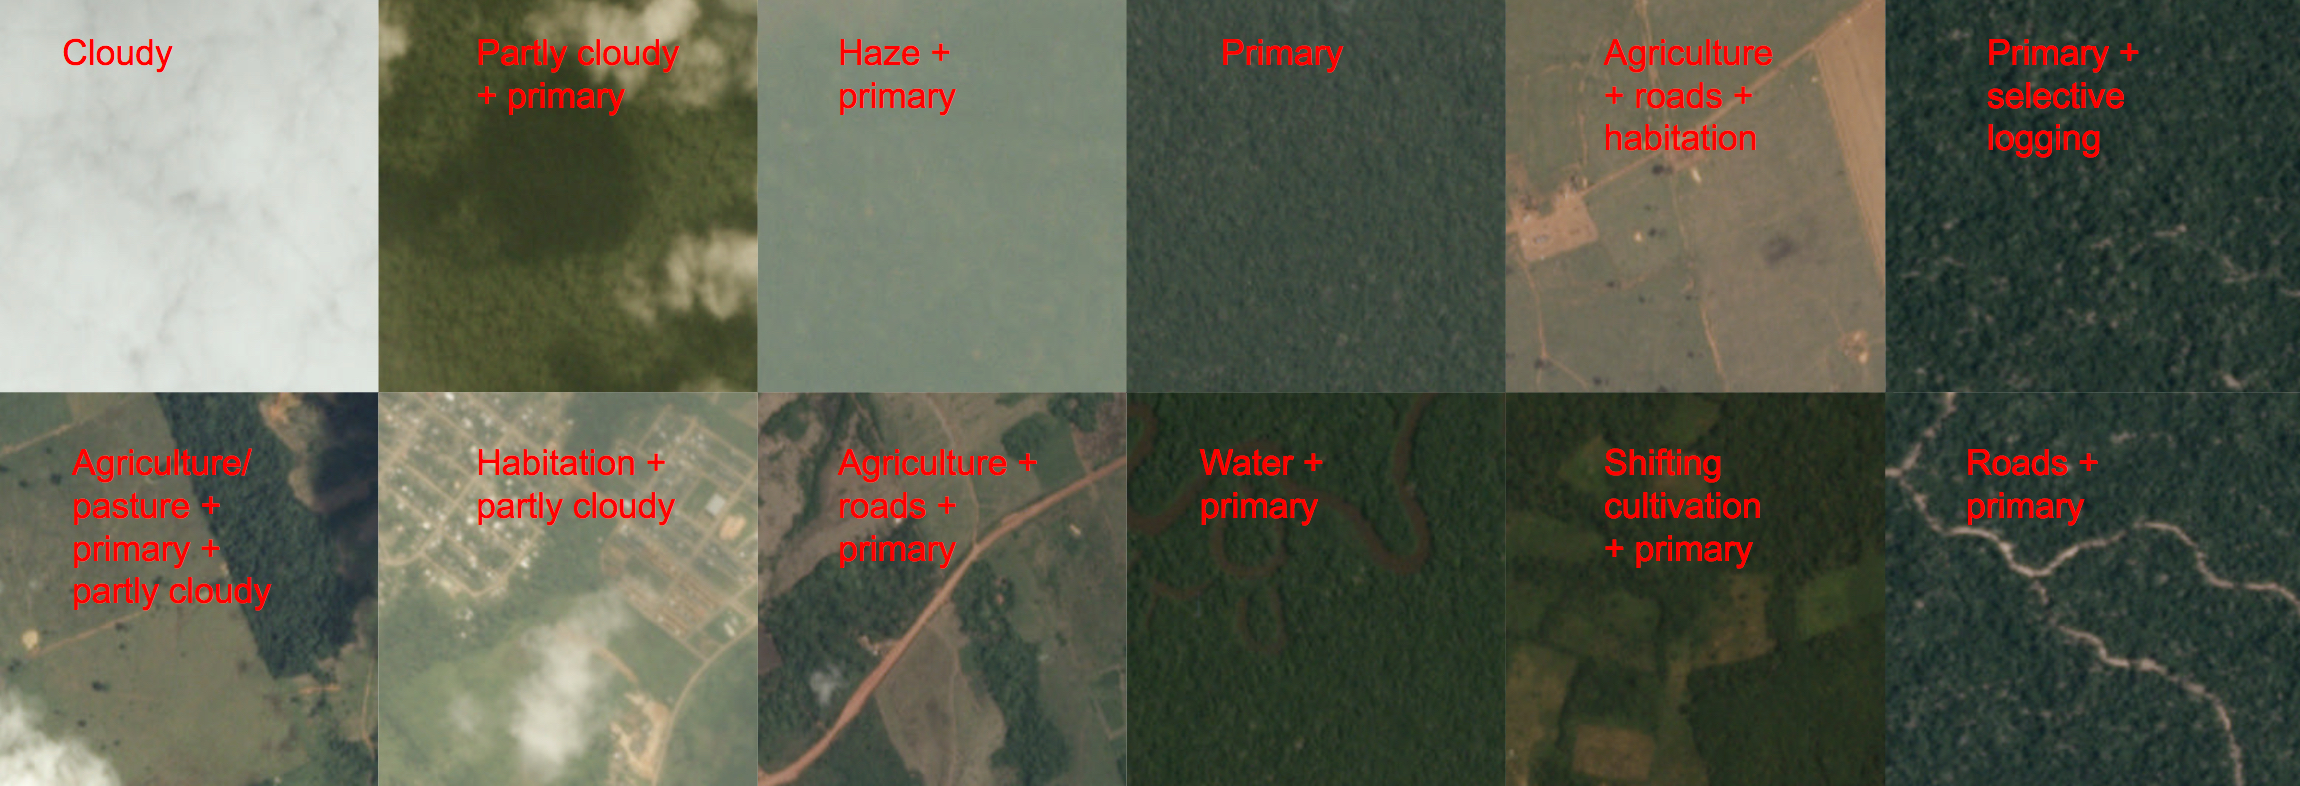
\includegraphics[width=0.9\columnwidth]{
        Imagens/chips.jpg
    }
    \caption{Amostras de classes do dataset Amazônia do Espaço}\label{fig:dataset}
\end{figure}

%We utilize a dataset (URL: https://www.kaggle.com/c/planet-understanding-the-amazon-from-space/data) published in a Kaggle competition (by Planet company), containing coarse-resolution imagery data from satellites with varying spatial resolution characteristics, i.e., the imagery has a ground-sample distance (GSD) of 3.7 m and an orthorectified píxel size of 3 m. The data comes from Planet’s Flock tow satellites in both Sun-synchronous and ISS orbits and was collected in the time interval between January 1, 2016, and February 1, 2017. All of the images are derived from the Amazon basin. Mangrove deforestation in the Amazon forest is an intense phenomenon, and a plethora of factors that contribute to deforestation is observed there. Each entry contains imagery data in RGB plus the infrared band in geo-referenced.tiff format. In our experiment, the images are classified into 14 classes and the labels are broken into three groups: atmospheric conditions, common land cover/land use phenomena, and rare land cover/land use phenomena (see Fig. 3). Here, each entry is assigned to one or more classes.


\subsection{Dataset poças de garimpo}\label{sec:Cap2_amazonia_garimpo}

Este \textit{dataset} foi utilizado em \cite{rs14071746}, mencionado no capitulo anterior. Concerne a tarefa de identificação de mudanças de imagem. Aplicadas a identificação de garimpo artesanal de ouro de pequena escala; Pode ser desafiador de se identificar, dado a variabilidade de condições atmosféricas e baixa resolução. Foram utilizadas imagens de Madre de Dios, região do Peru. Bem como amostras de outros países: Venezuela, Indonésia e Myanmar. 

% (Verificar se esse dataset é utilizável para tarefa de classificação; Resolução parece muito baixa e área muito grande)

% Abstract: Monitoring changes within the land surface and open water bodies is critical for natural resource management, conservation, and environmental policy. While the use of satellite imagery for these purposes is common, fine-scale change detection can be a technical challenge. Difficulties arise from variable atmospheric conditions and the problem of assigning píxels to individual objects. We examined the degree to which two machine learning approaches can better characterize change detection in the context of a current conservation challenge, artisanal small-scale gold mining (ASGM). We obtained Sentinel-2 imagery and consulted with domain experts to construct an open-source labeled land-cover change dataset. The focus of this dataset is the Madre de Dios (MDD) region in Peru, a hotspot of ASGM activity. We also generated datasets of active ASGM areas in other countries (Venezuela, Indonesia, and Myanmar) for out-of-sample testing.


% Dataset Description

%- Understanding the Amazon from Space [20] — multilabel dataset to track the human footprint in the Amazon rainforest; we’ll mostly refer to this as the Amazon dataset.
%WiDS Datathon 2019 [21] — binary dataset for oil palm plantation detection in Borneo; we’ll mostly refer to this as the oil palm dataset.
% Towards Detecting Deforestation [22] — binary dataset for detecting coffee plantations in the Amazon rainforest; we’ll mostly refer to this as the coffee dataset.


% ----------------------------------------------------------

\section{\textit{Premissas}}\label{sec:Cap3_Premissas}

Temos que o problema de identificação em sensoriamento remoto impõe a dificuldade de alta similaridade extra-classes e divergências intra-classes, da qual surge uma dificuldade de generalização e de viés indutivo para identificação de amostras fora das classes treinadas. Temos ainda que o treinamento de tais modelos envolvem um volume massivo de amostras rotuladas. 


% ----------------------------------------------------------

\section{\textit{Proposta de solução}}\label{sec:Cap3_Proposta}

Como solução para o problema, foi proposta a utilização de um modelo de \textit{transformer visual}  pré-treinado em um conjunto de dados expressivo e realizar o \textit{fine-tune}\footnote{Ajuste fino} para o conjunto de dados de interesse. Dessa forma, obtendo um modelo com boa capacidade de generalização e melhor viés indutivo, assim demandando menor quantidade de amostras para ser treinado.

Para solucionar o problema de generalização e conjunto de dados limitado da região de interesse, propomos a utilização de um modelo pré-treinado explicado em~\ref{sec:Cap2_transfer} um dataset extensivo de imagens aéreas e de satélites, de forma a aproveitar seu extrator de características, como é realizado em~\cite{wang2022empirical}. Assim o modelo será re-treinado (\textit{fine tunning}) para a região de interesse mantendo os pesos das camadas de encoder otimizar apenas a camada MLP fortemente conectadas, assim como a camadas de saídas softmax. 

Dessa forma, a arquitetura proposta é o ViT apresentado em~\cite{wang2022empirical}
composta por camadas hierarquicas de encoders transformers  que funcionam como extratores de características. As camadas seguintes são camadas totalmente conectadas seguidas por uma camada \textit{softmax} que realiza a classificação.
% ----------------------------------------------------------

\section{\textit{Ambiente e ferramentas}}\label{sec:Cap3_Ferramentas}


O Ambiente dos experimentos será em cadernos \textit{Jupyters}, para ser facilmente replicável e ser executável em nuvem, com a possibilidade de alugar recursos computacionais da plataforma em nuvem \textit{Google Colab}. Também será utilizado o \textit{framework PyTorch}, por razões de disponibilidade de métodos e conhecimentos do autor. 

\subsection{\textit{Ambiente}}\label{sec:Cap2_Ambiente}

Foram dispostos 100h de orçamento de recursos computacionais, em uma instância da plataforma com GPU NVidia Tesla T4 de 12 GB de RAM. CPU Intel(R) Xeon(R) CPU @ 2.20GHz, 12 GB de memória. Para o treinamento de redes neurais profundas, aceleradores como placas gráficas podem resultar em ganhos de tempo de até 40x em com paração com treinamentos em CPU, bem como o uso da ram para placa gráfica para realizar \textit{caching}\footnote[1]{Uma cache é um bloco de memória para o armazenamento temporário e ágil de dados que possuem uma grande probabilidade de serem utilizados novamente} obtendo melhores tempos de acesso durante carregamentos.


\subsection{\textit{Bibliotecas}}\label{sec:Cap2_NumpyPandas}

Para o experimento também contou-se com bibliotecas de calculo numérico e algébrico como o Numpy. Também Pandas para manipulação de dados tabulares. Já a ferramenta SciKitLearn contém diversos módulos para aprendizado estatístico, como funções de métricas, de perdas. Para visualização dos resultados utilizado serão MatplotLib, Plotly e Seaborn.

\subsection{\textit{PyTorch}}\label{sec:Cap2_PyTorch}
Pytorch é um \textit{framework}\footnote{Ferramental} código aberto de de front-end em Python para aprendizado profundo. É implementado em linguagens C++ e CUDA para otimizações de computações numéricas e matriciais, que são extensivas para esta aplicação.
O projeto é originalmente criado pelo \textit{Facebook Research} e é atualmente amplamente adotado pela academia e mercado em aplicações de aprendizado profundo. Possui muitas implementações das ferramentas mais utilizadas, especificamente aplicadas a \textit{Deep Learning} e visão computacional. Tem ampla adoção devido à intenção de ser um \textit{framework} de fácil uso e alto nível, com muitas abstrações e técnicas já implementadas.

% ----------------------------------------------------------


% TODO: citar o paper de aplicação direta
\section{\textit{Experimentos}}\label{sec:Cap3_Experimentos}

Para a construção da solução desejada, experimentaremos combinar um modelo pré-treinado com camadas internas, correspondente ao extrator de características e de saída treinadas para a região de interesse.
Consiste em fazer experimentos em uma complexidade crescente, e replicando resultados para garantir corretude. Será simplificado a reprodução para apenas um \textit{dataset}.


Para obter o modelo proposto e de melhor desempenho, inicialmente define-se os seguintes passos de experimentos para construir o modelo final:

\begin{enumerate}
\item   Análise exploratória dos dados, visando a melhor conhecer o problema e amostras. 
\item   Replicar experimentos dos trabalhos~\ref{sec:Cap2_million} com \textit{checkpoints}\footnote{Captura dos pesos de uma rede a partir de certo ponto do processo de treino} disponibilizados, a fim de replicar a metodologia de fine-tune. 
\item   Replicar experimentos de \ref{sec:Cap2_ForestViT} em um modelo base de comparação baseado em em uma CNN ResNet-50
\item   Criar um modelo baseline RESNET, fazendo ajuste de hiperparâmetros a fim de obter o melhor score no baseline
\item   Realizar o mesmo para o modelo de transformers visuais
\item   Fixar os hiperparâmetros e metodologia de treino para ambos modelos e treiná-los novamente
\item   Realizar análise dos resultados de ambos e comparar performance em várias métricas
\item   Avaliar desempenho, comparar com os experimentos e trabalhos bases \ref{sec:Cap2_revisao_literatura}
\end{enumerate}


    
% ----------------------------------------------------------

\section{\textit{Procedimentos}}\label{sec:Cap3_Procedimentos}

Os procedimentos do experimento principal consiste principalmente nas etapas de configuração do ambiente, pré-processamento do conjunto de dados, análise exploratória, definição do modelo e iterações de treino-validação. Explicadas adiante.

\subsection{\textit{Configuração de Ambiente}}\label{sec:Cap3_ConfigAmbiente}

A plataforma GoogleColab consiste em uma instancia alocada temporariamente com custo por tempo de uso, porém com desconexão por tempo ocioso. Durante o treinamento a interface se torna ociosa e ocorrem desconexões. Para mitigar isto foram criadas funções de gerenciar contexto do experimento, para implementar o armazenamento e carregamento se estatisticas do treinamento a cada epoch.

Os arquivos compactados de são obtido de hospedagem em nuvem e descompactado na instância, seja em disco ou em partição na memória ram. Esta segunda opção permitiu importantes melhorias de tempo de carregamento de batches. O arquivo contendo os pesos do modelo para criação do modelo são obtidos da mesma forma. Com cada instância é volátil, sendo possível armazenar conteúdos somente no serviço de hospedagem GoogleDrive, os resultados, pesos do modelo e contexto do experimento precisam ser salvos a cada execução, em caso de desconexão.


O pré-processamento em cada amostra é feito em tempo de execução por instâncias de transformação composta de:
\begin{enumerate}
    \item   Carregamento de cada imagem dos canais RGB e discartando o infravermelho-próximo
    \item   Redimensionamento usando interpolação linear de $256 \times 256px$ para $224 \times 224px$. Isto se deve ao fato dos modelos já terem sido pré-treinados e configurados para essa dimensão de entrada.
    \item   Conversão da imagem para estrutura de dados numérica de Tensor
    \item   Aplicar espelho vertical ou horizontal, cada um com probabilidade de 25%.
    \item   Normalizar cada canal de cor RGB usando normalização Gaussiana com médias e desvio padrão do dataset ImageNet.
\end{enumerate}



\subsection{\textit{Análise de dados exploratória}}\label{sec:Cap3_AnaliseDeDadosExploratoria}
Para melhor entendimento das características do conjunto de dados, se faz necessário uma exploração dos dados. Consiste em entender os diferentes tipos de amostras e rótulos, por meio de estatísticas de distribuição de classes e visualizações de agrupamento.



Pela distribuição de classes em , podemos observar que se trata de um dataset com acentuado desbalanço. 

\begin{table}[h!]
    \caption{Delay Comparison of Proposed and Existing Method}
    \centering
\begin{tabular}{*{4}{c}}
    \toprule
    Classe                  &            Rótulo &  Cardinalidade &  Proporção (\%) \\
    \midrule
    Mina Convencional       & conventional mine &    100 &       0.247 \\
    Roça de Ventos          &         blow down &    101 &       0.250 \\
    Queimada                &        slash burn &    209 &       0.516 \\
    Florescimento           &          blooming &    332 &       0.820 \\
    Garimpo                 &    artisinal mine &    339 &       0.837 \\
    Desmatamento Seletivo   & selective logging &    340 &       0.840 \\
    Área Desmatada          &       bare ground &    862 &       2.129 \\
    Nublado                 &            cloudy &   2089 &       5.161 \\
    Névoa                   &              haze &   2697 &       6.663 \\
    Habitação               &        habitation &   3660 &       9.042 \\
    Cultivação              &       cultivation &   4547 &      11.233 \\
    Parcialmente Nublado    &     partly cloudy &   7261 &      17.938 \\
    Água                    &             water &   7411 &      18.308 \\
    Estrada                 &              road &   8071 &      19.939 \\
    Agricultura             &       agriculture &  12315 &      30.423 \\
    Clima Limpo             &             clear &  28431 &      70.236 \\
    Vegetação Primária      &           primary &  37513 &      92.673 \\
    \bottomrule
\end{tabular}
\label{tab1}
\end{table}

Na figura \ref{fig:classes} a seguir podemos visualizar amostras de cada tipo de classe. Cada amostra pode pdertencer a mais de um tipo de classe.


\begin{figure}[!ht]
    \centering
    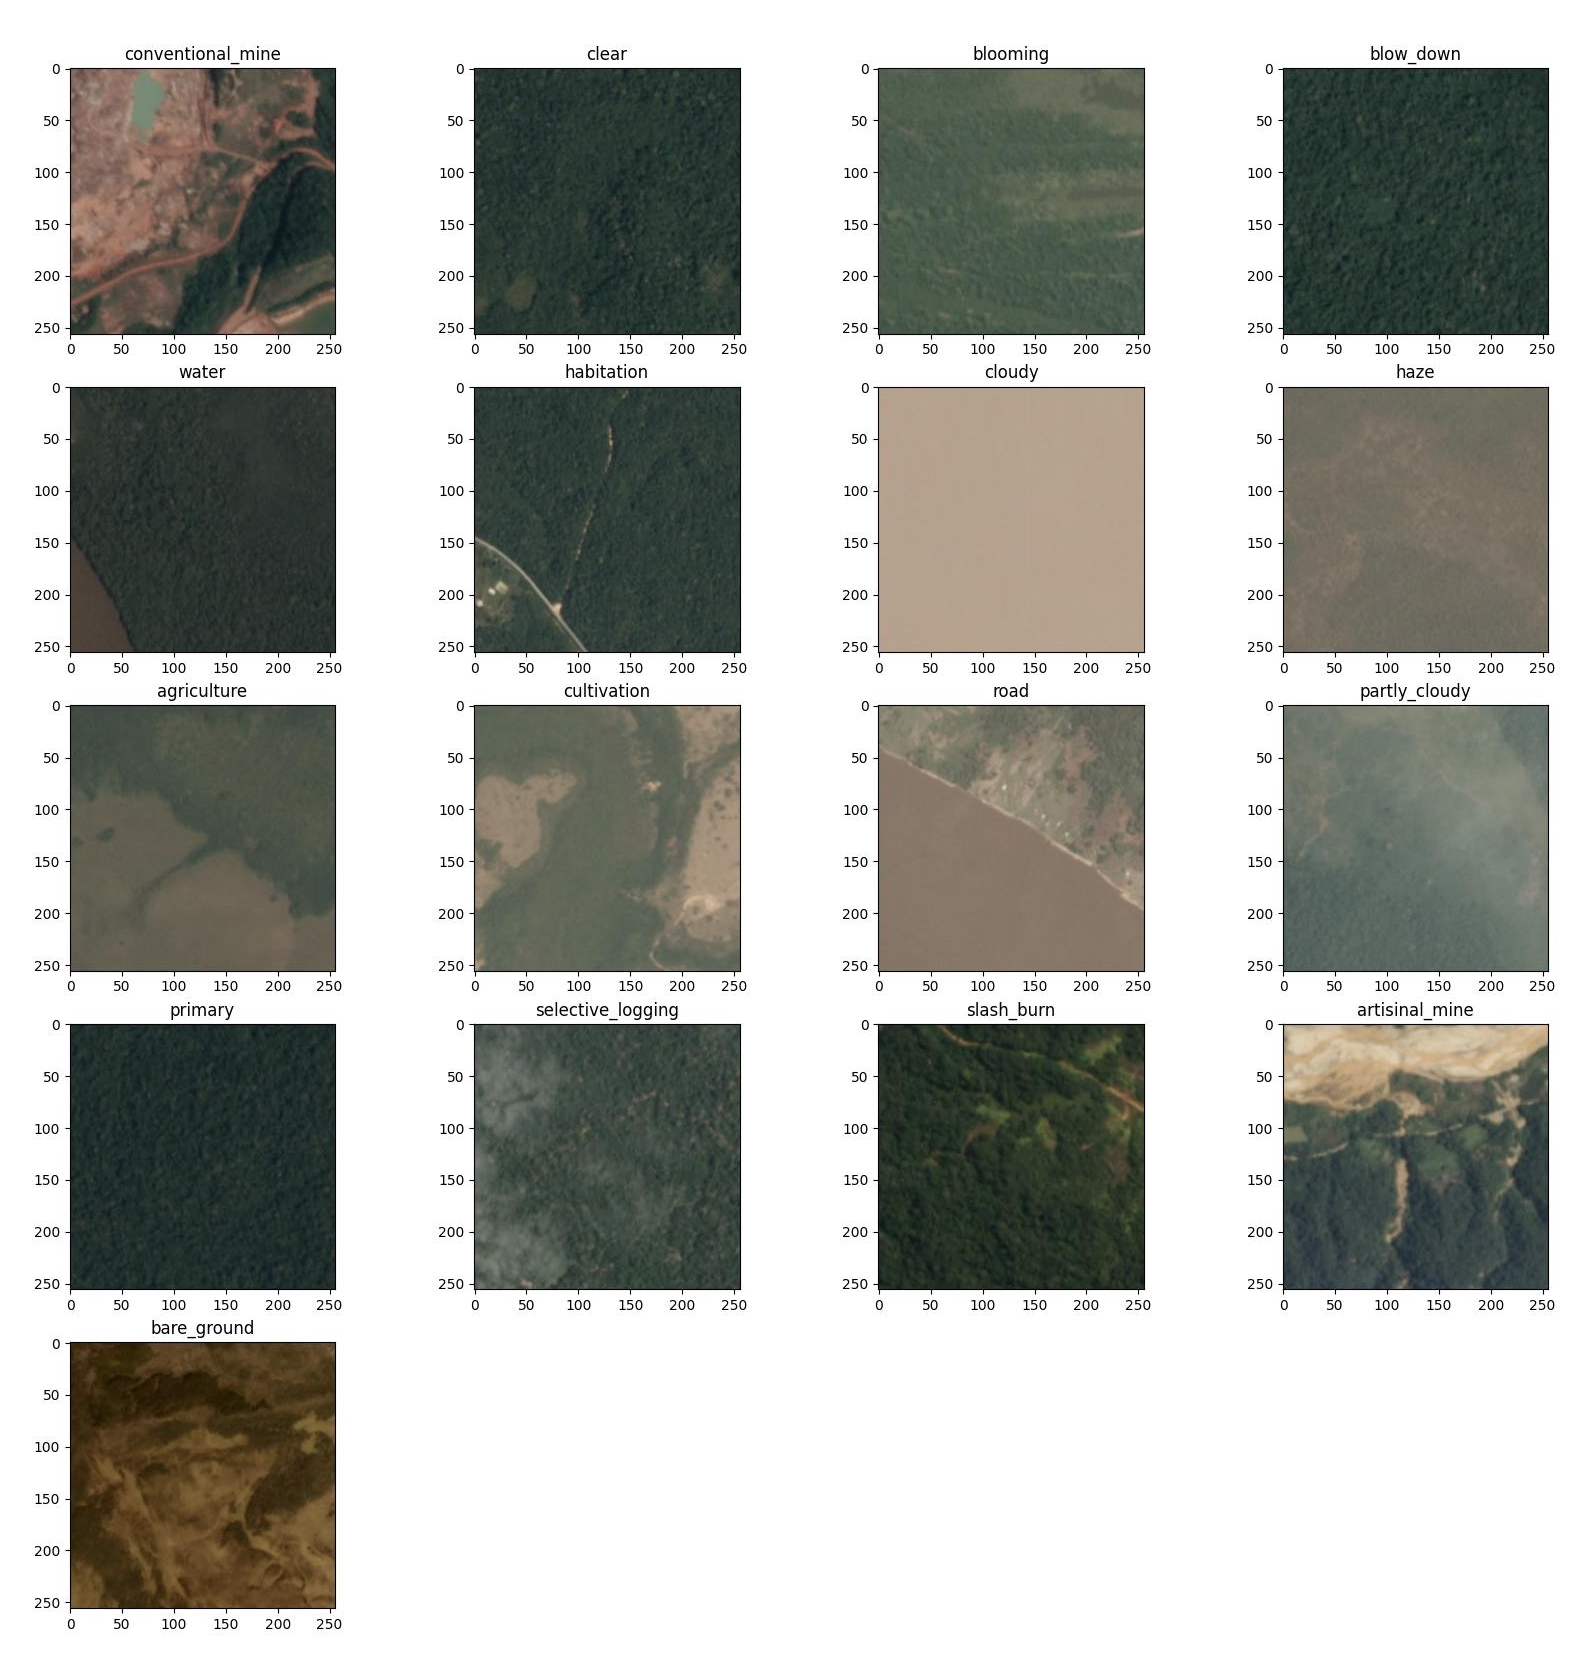
\includegraphics[width=\columnwidth]{Imagens/results/EDA/Class Sampling.jpg}
    \caption{Amostragem de cada classe de rótulo.
    Fonte: Autor}
   \label{fig:classes}
\end{figure}

%\begin{figure}[!ht]
%    \centering
%    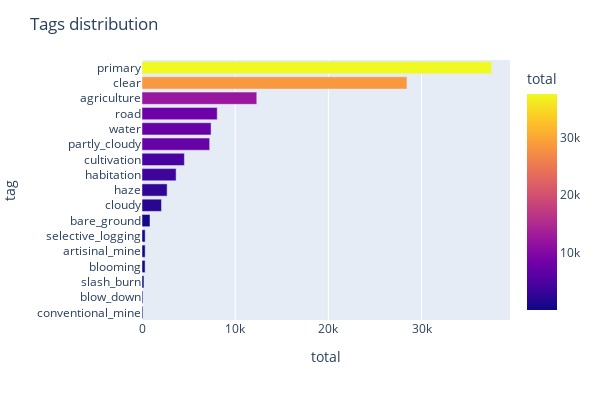
\includegraphics[width=0.9\columnwidth]{Imagens/results/EDA/Class distribution.jpg}
%    \caption{Distribuição da quantidade de amostras por classe.
%    Fonte: Autor}
%   \label{fig:classes_distribuicao}
%\end{figure}

\begin{figure}[!ht]
    \centering
    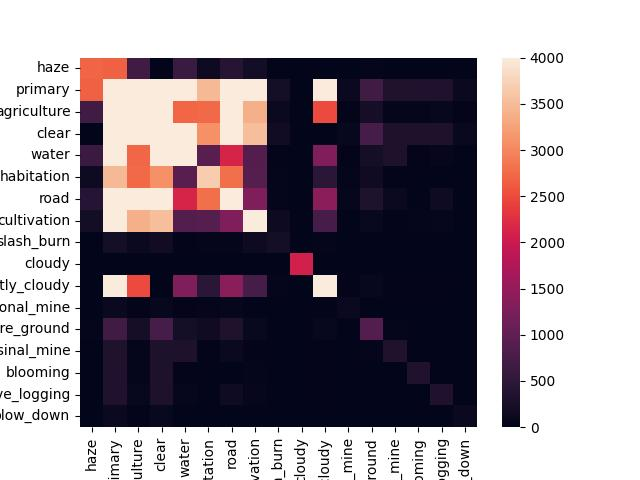
\includegraphics[width=0.5\columnwidth]{Imagens/results/EDA/Co-occurrence matrix.jpg}
    \caption{Matriz de co-ocorrência.
    Fonte: Autor}
   \label{fig:coocorrencia}
\end{figure}

\begin{figure}[!ht]
    \centering
    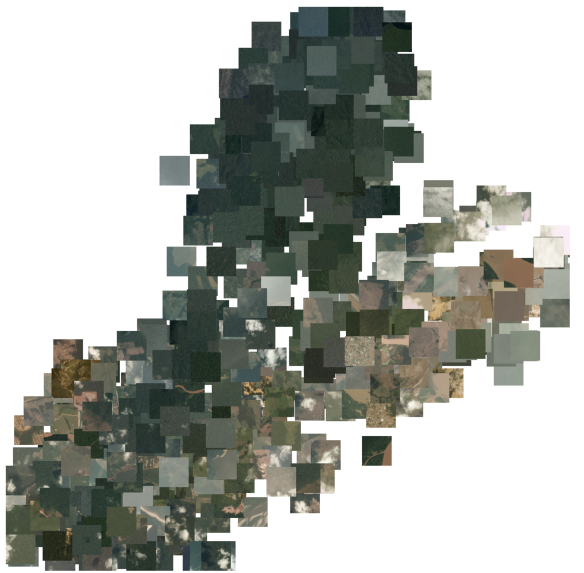
\includegraphics[width=0.9\columnwidth]{Imagens/results/EDA/TSNE.png}
    \caption{Agrupamento de amostras via técnica TSNE.
    Fonte: Autor}
   \label{fig:TSNE}
\end{figure}

\subsection{\textit{Pré-processamento}}\label{sec:Cap3_PreProcess}
O pré-processamento consiste em preparar as amostras do conjunto de dados de interesse para treino e validação. Para o conjunto de dados floresta amazônica temos 40000 amostras. Foram separadas em uma divisão de treino-teste na proporção 80\%-20\%. Cada recorte de resolução $256 \times 256$ px.


\subsection{\textit{Definição do modelo}}\label{sec:Cap3_Def_modelo}


% TODO Imagem da arquitetura proposta.
\begin{figure}[!ht]
    \centering
    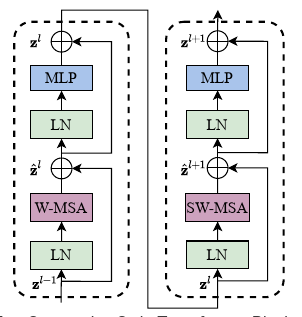
\includegraphics[width=0.5\columnwidth]{Imagens/dois blocos swin sucessivos.png}
    \caption{ Arquitetura de modelo proposta.
    Fonte: Autor}
   \label{fig:Swin-Rsp}
\end{figure}

% TODO Imagem da arquitetura proposta.
\begin{figure}[!ht]
    \centering
    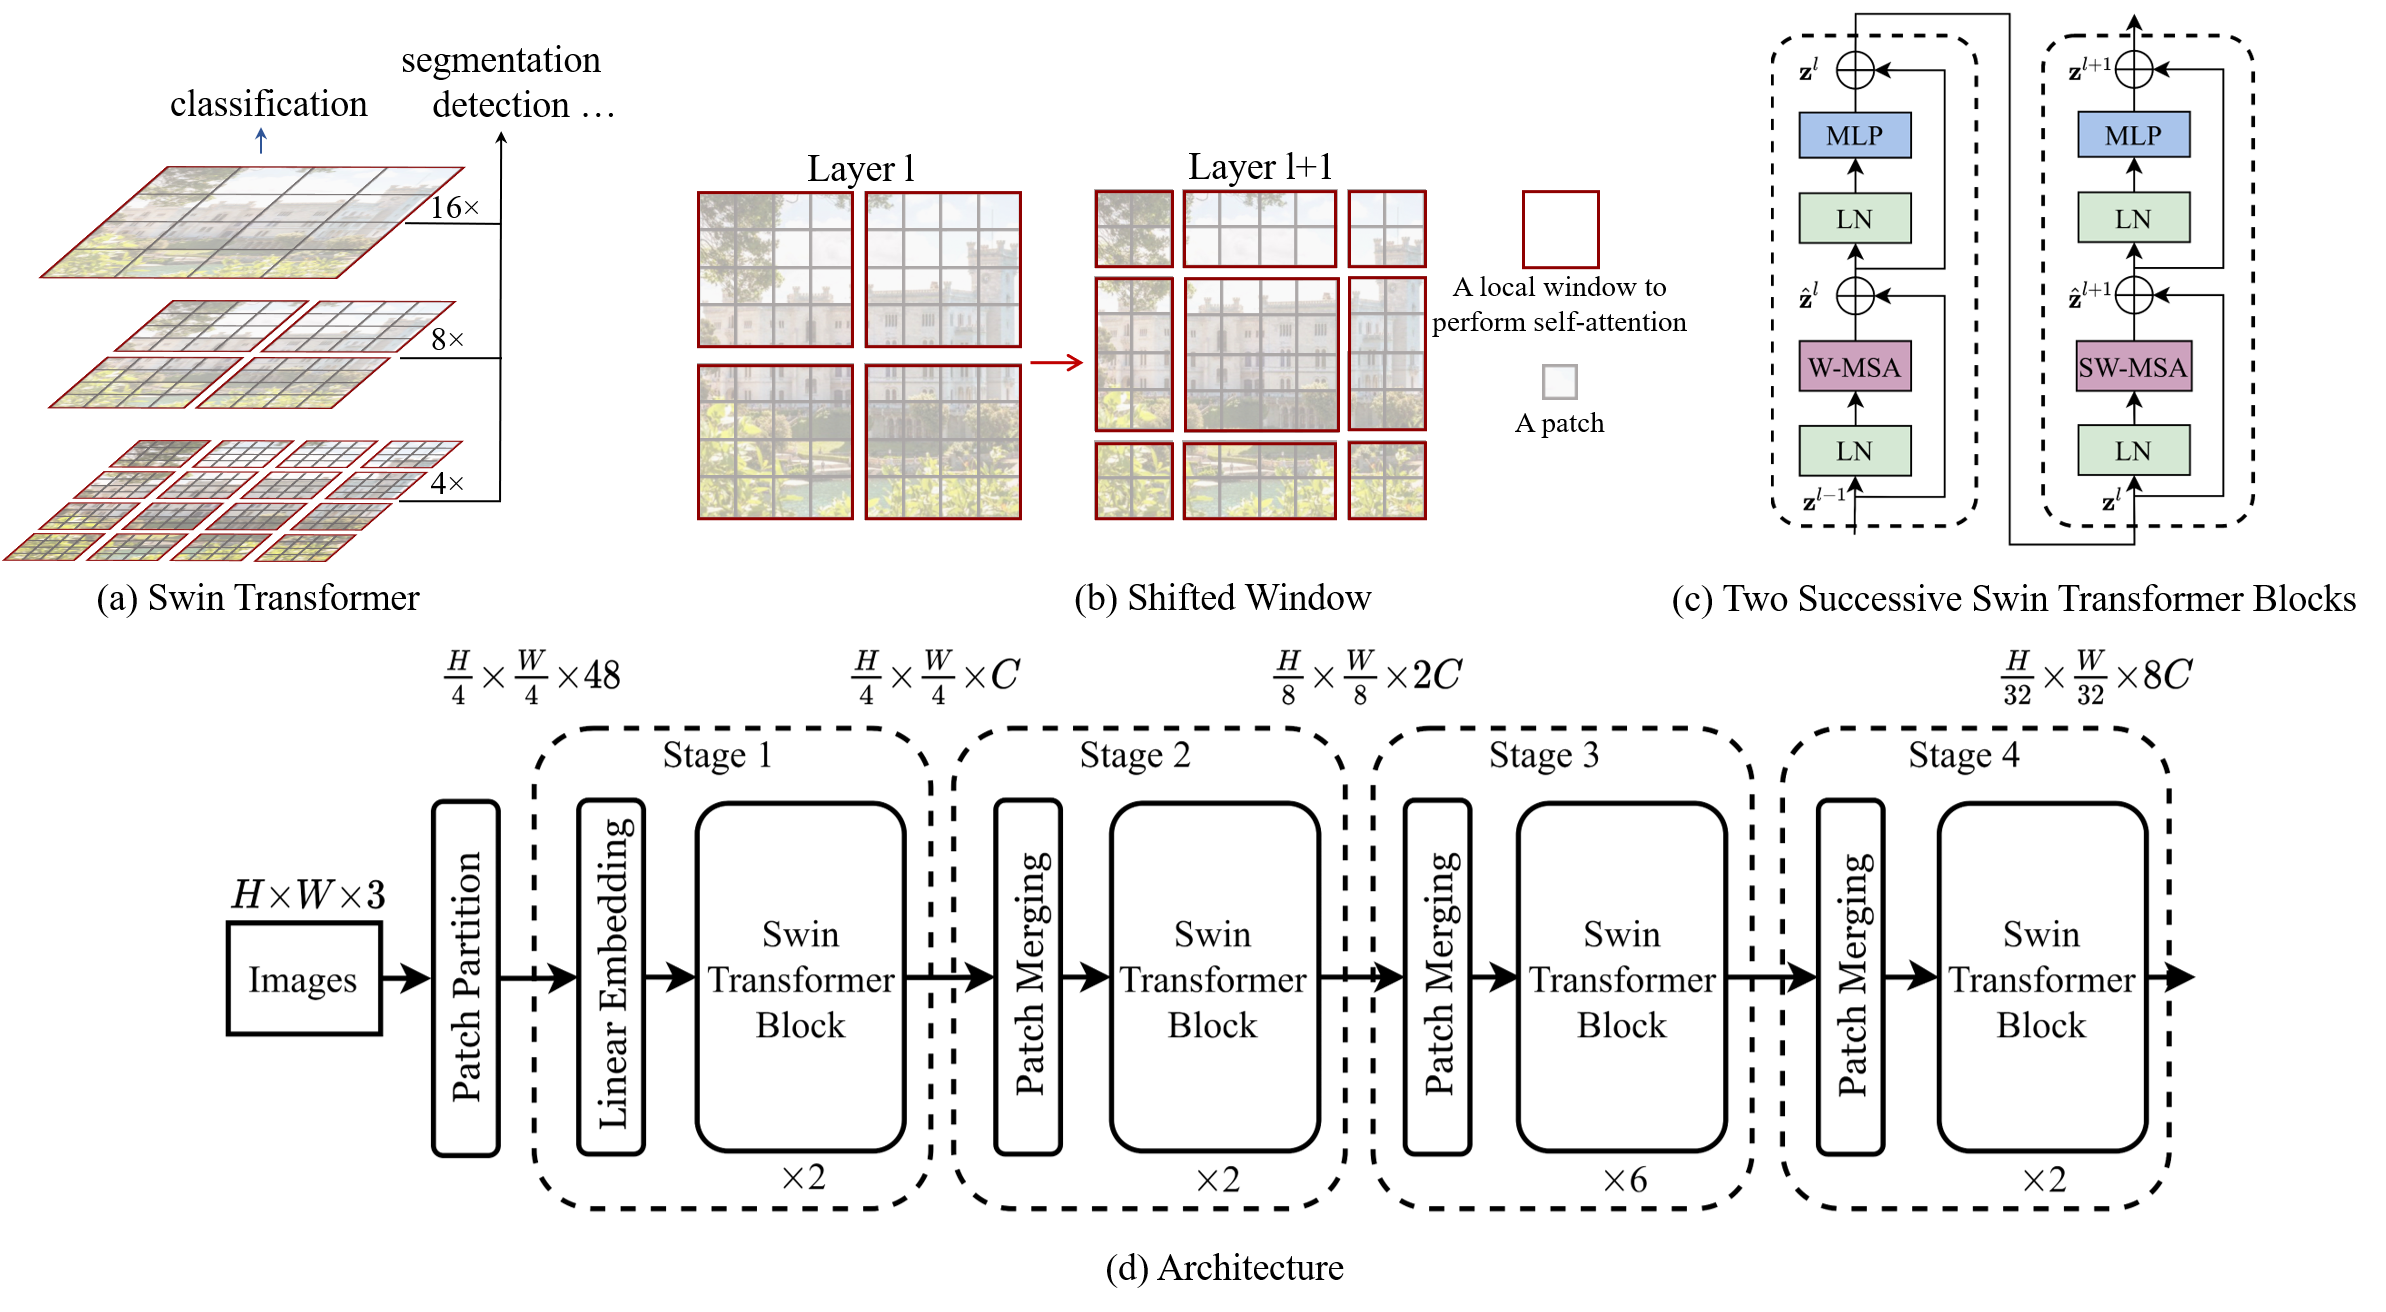
\includegraphics[width=0.9\columnwidth]{Imagens/arquitetura swin.png}
    \caption{ Arquitetura de modelo base.
    Fonte: Autor}
   \label{fig:ResNet-Rsp}
\end{figure}




\subsection{\textit{Treino}}\label{sec:Cap3_Treino}

Para a etapa de treino, utilizamos a arquitetura proposta em~\ref{sec:Cap3_Proposta}, que consiste em um modelo pré-treinado, e retreinando suas ultimas camadas de classificação por camadas fortemente conectadas seguidas de camadas de \textit{softmax}, como ilustra a imagem a seguir:


\subsection{\textit{Validação}}\label{sec:Cap3_Validacao}

A etapa de validação será realizada a medida do desempenho do modelo no conjunto de testes para classificação.

